\chapter{Implémentation}

\section{Logotiel}
Le logitiel développer dans le cadre de ce travail à pour objectif de communiquer avec le capteur QCM, traiter, afficher les données collectés et sauver les donnée collecter.
Le logitielc fourni par le fabriquant contient permet deja d'utiliser le capteur. cependant il manquait certaine fonctionnalité tel que s'ouvir en une seul fenêtre,
avoir total contrôle sur les mesures c'est a dire pouvoir changer la precision ainsi que ma largeur de la messure en Hz. 
Il est aussi possible de choisisr non seulement quel harmonique on desire mesurer mais il est possible de choisir plusieurs a mesurer en meme temps.
\subsection{architectures du Logitiel}
Le programmes utilise une architecture orienter object. chaque object a une responsablilté. L'object Serial s'occupe de la communiction avec la balace. Il est responssable de la connection, de lire les sorties et de mettre en forme les données recus.
L'object signal lui s'occupe des signeux une fois recu dans le C'est cet object qui s'occupe de faire le traitement du signal. Parameter contiens tous les paramètre pour chaque signal. L'object mesure petremet de faire le lient entre les diferent object. ilt est responsable de toute la mesure. 
\fig[H, width=12cm]{Diagramme de classe}{uml.drawio}

\subsection{Mesures}
Les mesures se déroulent en deux étapes.
Dans un premier temps, le capteur effectue une mesure de calibration. Cette mesure consiste à balayer toute la plage de fréquences allant de 1 à 5,5 MHz \ref{fig:calibration plot}.
L’objectif de cette étape est d’identifier automatiquement les fréquences de résonance du quartz. Pour ce faire, il est essentiel de détecter la fréquence fondamentale du quartz afin de déterminer s’il s’agit d’un quartz 10 MHz ou 5 MHz.
La méthode consiste à repérer la position du premier pic de résonance. Une fois cette fréquence déterminée, le programme peut ensuite rechercher toutes les fréquences de résonance : on en attend trois pour un quartz à 10 MHz et six pour un quartz à 5 MHz.

\begin{figure}[H]
    \centering
    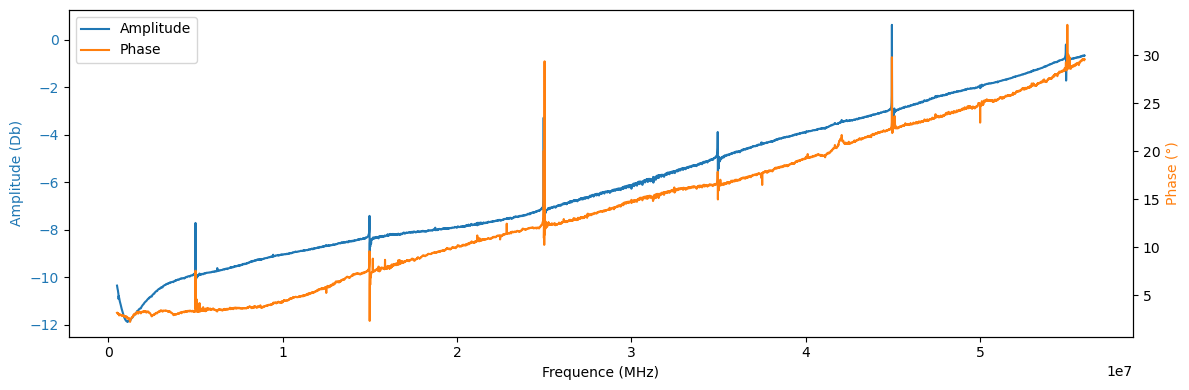
\includegraphics[width=\textwidth]{assets/figures/Calibration.png}
    \caption{Signal de calibration du capteur QCM comportant 6 pics de résonance.}
    \label{fig:calibration plot}
\end{figure}
La deuxième étape consiste à Mesurer plus précisement les pics de résonance figure~\ref{fig:harmonic plot} trouver lors de la mesure de callibration. Pour faire cela une fenetre est choisis autour de chaque pic de raisonnace le pas de mesure est aussi très fortement diminuer pour une précision maximale.
\begin{figure}[H]
    \centering
    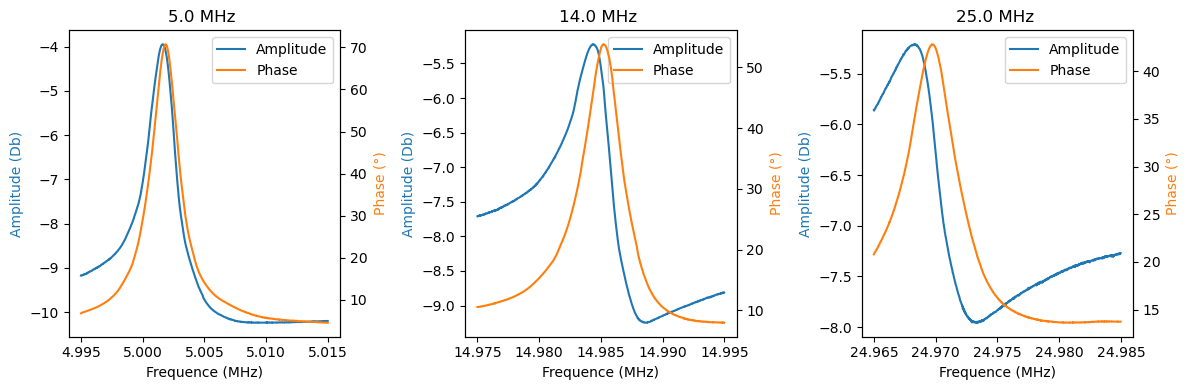
\includegraphics[width=\textwidth]{assets/figures/signalpeak.png}
    \caption{Signal des 3 premières harmoniques de résonance.}
    \label{fig:harmonic plot}
\end{figure}

\subsection{selection des mesures}
Depuis le menu il est possible d'accéder a la fenetre de sélection des paramètres de mesure \ref{fig:paramerter window}.
Les paramètres suivant peuvent être modifier par l'utilisateur celon ses besoins.
\begin{itemize}
    \item \textbf{Activation d'une limites de mesure} : Si une limite de mesure est activée, la mesure s'arrêtera lorsque cette limite sera atteinte.
    \item \textbf{Limite du nombre de mesures} : Le nombre maximum de mesures à effectuer.
    \item \textbf{pas de la messure de calibration} : Le pas de mesure en Hz pour la mesure de calibration.
    \item \textbf{décalage negatif de la des mesures de peak}: Le décalage négatif à appliquer aux mesures de pic.
    \item \textbf{décalage positif de la des mesures de peak}: Le décalage positif à appliquer aux mesures de pic.
    \item \textbf{pas des messures de peak} : Le pas de mesure en Hz pour les mesures de pic.
    \item \textbf{harmonique} : La ou les harmoniques à mesurer. Il est possible de sélectionner plusieurs harmoniques.
    \item \textbf{temps d'attente}: Le temps d'attente entre chaque mesure en secondes.
    \item \textbf{Calibration par la phase} : Si cette option est activée, la calibration se fera en fonction de la phase du signal. sinon la calibration se fera en fonction de l'amplitude du signal.
\end{itemize}

\begin{figure}[H]
    \centering
    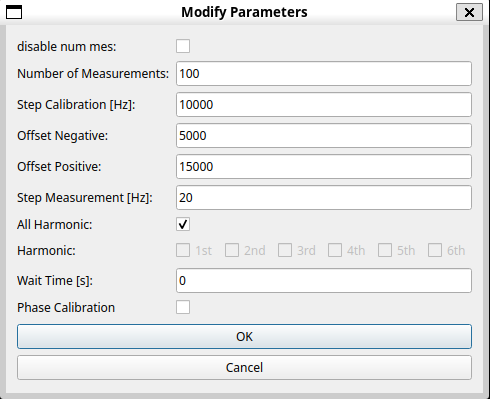
\includegraphics[width=0.6\textwidth]{assets/figures/Parameter_window.png}
    \caption{Fenetre de selection des paramètres de mesure}
    \label{fig:paramerter window}
\end{figure}

\subsection{affichage des données}
Le logiciel dispose de plusieurs fenêtres pour afficher les données.
La première est la fenêtre de mesures figure~\ref{fig:main window} qui est composer d'une barre d'outil sur le dessus qui contiens tous les contrôles nessecaire a contrôler les mesures.
Sur la droite une liste permet de visualiser l'ensemble des baches mesurer ainsi que les paramètre associer.
A gauche une section est réserver pour les graphiques. cette zone est séparer en trois partie:
\begin{itemize}
    \item La partie supérieure affiche les signaux d'amplitude et de phase du signal de calibration.
    \item La partie centrale affiche les signaux d'amplitude et de phase des harmoniques mesurées. Ce groupe est dynamique selon le nombre d'harmoniques choisies.
    \item La partie inférieure affiche la fréquence de la première harmonique mesurée en fonction du temps. Ainsi que la température du capteur intégré.
\end{itemize}

La deuxième fenêtre est la fenêtre de visualisation des données figure~\ref{fig:plot window}. 
Elle permet de visualiser les données mesurées sous forme de graphique. 
Il est possible de choisir n'importe quelle paramètre de la mesure à afficher sur l'axe de abscisse et n'importe quel paramètre de la mesure à afficher sur l'axe des ordonnées.
Il est aussi possible de choisir l'harmonique à afficher.
\begin{figure}[H]
    \centering
    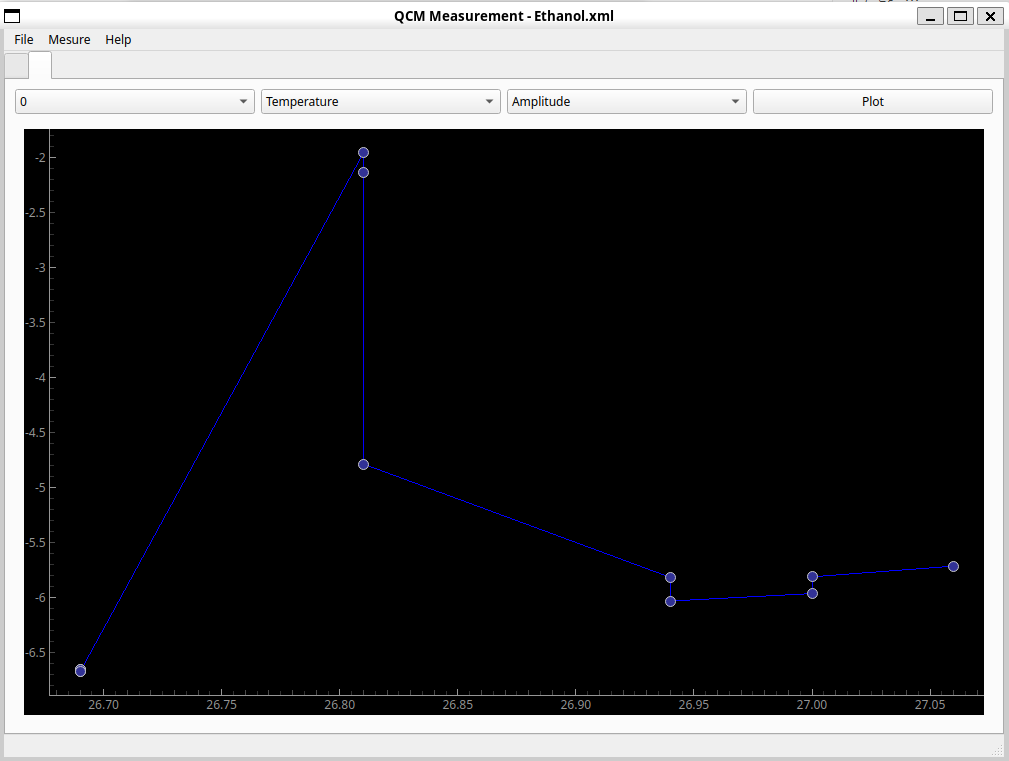
\includegraphics[width=0.8\textwidth]{assets/figures/Plot_window.png}
    \caption{Fenetre de visualisation des données}
    \label{fig:plot window}
\end{figure}
\begin{figure}[H]
    \centering
    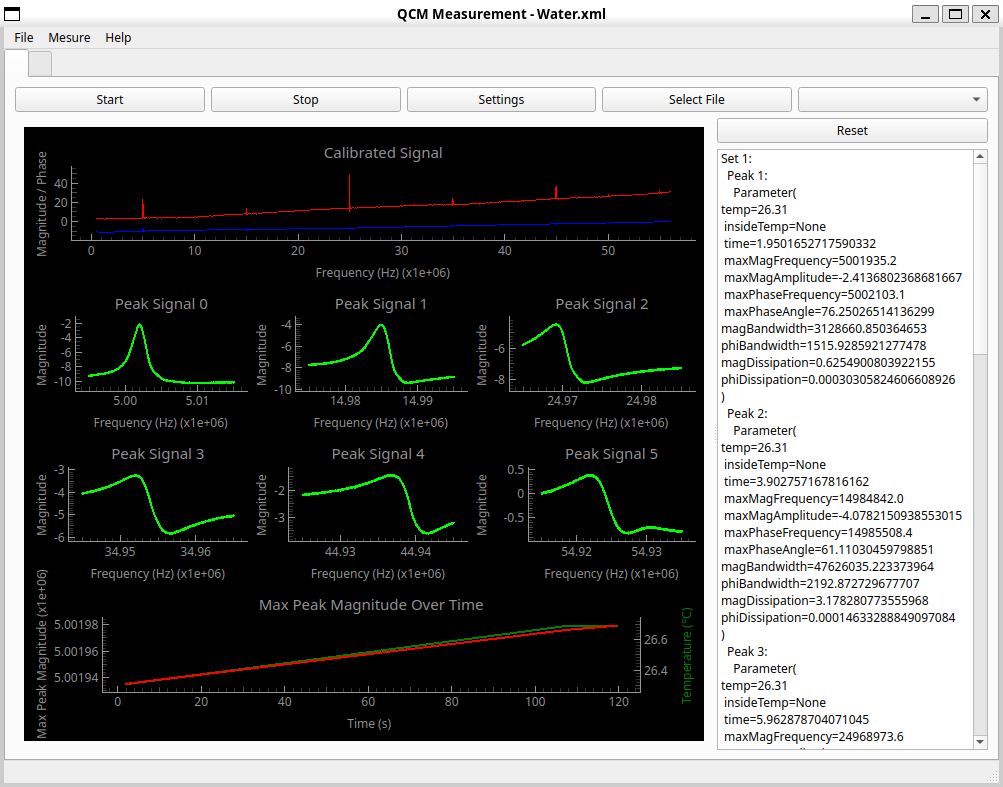
\includegraphics[width=0.8\textwidth]{assets/figures/Programme.png}
    \caption{Fenetre principale du logiciel de mesure}
    \label{fig:main window}
\end{figure}


\subsection{communication avec le capteur}
Pour communiquer avec le capteur une connexion sérielle est établie. cette connexion permet d'envoyer des commandes et de recevoir des données.

L'envoi des commandes est un string qui est envoyé. la commande comprend le la fréquence de debut la frequence de fin et le pas de la mesure. les données sont séparée par une semicolon (;). La tramme est terminée par un retours a la ligne (\texttt{\textbackslash n}).
\begin{minted}{bash}
500000;55990000;10000

9985000;10004980;20

29995000;30014980;20
\end{minted}
Le capteurs répond avec les donnée mesurée. Les donnée sont formattée avec l'amplitude en premier suivi par la phase et separer par un point virgule (;). les point de messure sont séparé par un retour a la ligne (\texttt{\textbackslash n}).
pour annoncer que la mesure est terminée le capteur envoie la temperatures en degrer celcus suivi par in point virgule (;) et un (s)

\begin{minted}{bash}
2968.94;3450.61\n

25.81;s
\end{minted}

La conversion des valeurs brutes issues de l'ADC en unités physiques se fait selon l'équation~\ref{eq:adc_conversion}.

\begin{equation}
A_i = \frac{\left( \left( x_i \times \frac{k}{2} \right) - V_{\text{CP}} \right)}{0.03}
\label{eq:adc_conversion_Amplitude}
\end{equation}

\begin{equation}
\phi_i = \frac{\left( \left( x_i \times \frac{k}{1.5} \right) - V_{\text{CP}} \right)}{0.01}
\label{eq:adc_conversion_phase}
\end{equation}

\begin{equation}
k = \frac{V_{\text{max}}}{N_{\text{max}}}
\label{eq:adc_conversion}
\end{equation}

où :
\begin{itemize}
    \item $x_i$ : valeur brute de l'ADC pour l'échantillon $i$,
    \item $V_{\text{max}}$ : tension maximale mesurable par l'ADC (ici $3.3\,\mathrm{V}$),
    \item $N_{\text{max}}$ : valeur maximale du codeur ADC (ici $8192$ pour un ADC sur 13 bits),
    \item $V_{\text{CP}}$ : tension de référence (0.9),
    \item $y_i$ : valeur convertie (en unité physique finale).
\end{itemize}

\section{traitement du signal}

\newpage

\section{Viscosité}
Pour effectuer les mesures de viscositer nous avons d'abord pris des mesures de la réponse fréquenciel du capteur dans plusieurs milieux.
afain de comparer les résultat avec les mesures de viscosité theorique des elements. Les elements choisis sont l'aire, l'eau distillée, l'éthanol et l'huile moteur.
\begin{table}[H]
    \centering
    \begin{tabular}{|l|c|}
        \hline
        \textbf{Élément}      & \textbf{Viscosité (mPa·s)} \\
        \hline
        Air                  & 0.018 \\
        Eau distillée        & 1.00  \\
        Éthanol              & 1.20  \\
        Huile moteur         & 150   \\
        \hline
    \end{tabular}
    \caption{Viscosité des différents éléments mesurés à température ambiante}
    \label{tab:viscosite_elements}
\end{table}
Ces elements ont été choisis pour leur grande différance de viscosité mais aussi pour leur disponibilité et leur faible dangerosité
Pour ce test le quartz utiliser est un quartz de 5MHz. La cellule Fluidic est utiliser sans pompe et le capteur est rempli de l'echantillon au moyen d'une ceringue. 
Aucun changement de temperature n'est effectuer pendant la mesure, ni aucune mesure de viscosité au moyen du viscomètre au laboratoire.
Ce test a pour vocation de montrer la façon dont la fréquence de résonance change en fonction de la viscosité du milieu dans lequel le quartz est immergé. Et de comparer avec les resultat theorique de viscosité de ces éléments.

\section{gestion de la température}
Avant de pouvoir faire de la gélatine il est essentielle de pouvoir refroidir le liquide à une temperature en dessous de 20 degrer pour que le processus de gelification commence. 
pour cela un bain de glace est utilisé. le liquide est mis dans le récipient en verre du module electrochimique. au moyen d'un tuyeaus et d'une pompe peristatique le liquide est circuler autour du recipient. le tuyeaux est enrouler autour du récipient afain de fcréer un echangeurs de chaleur.
\begin{figure}[H]
    \centering
    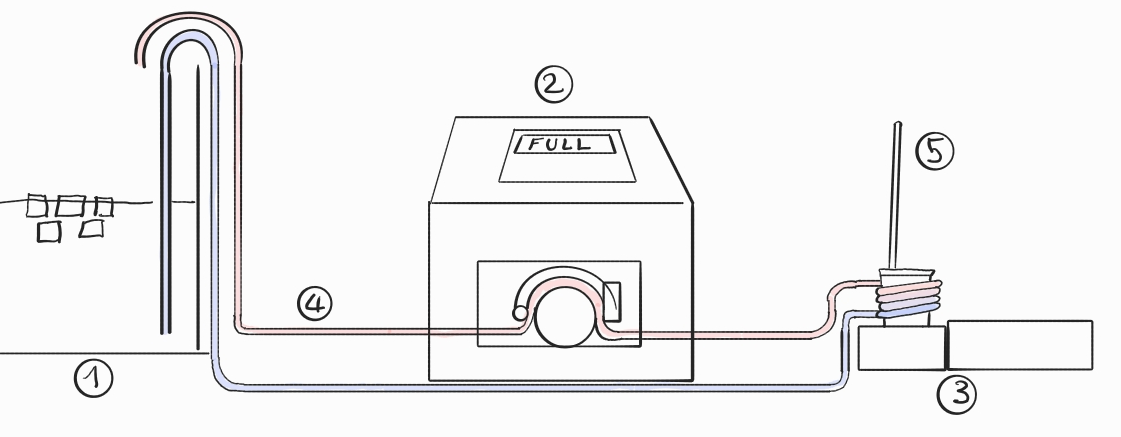
\includegraphics[width=\textwidth]{assets/figures/Pump TB.png}
    \caption{Shema de refroidissement du module QCM}
    \label{fig:Shema_glacière}
\end{figure}
Afain de chauffer le melange si une température plus haute que la temperature ambiante est nessecaire, le bac d'eau glacée est remplacer par un bain chauffant reglable.
Pour tenir le tuyeaux en place un clip a été designer et imprimer en 3D. le clip est composer de 4 section ce cercle qui permete de glicer le tyeau flexile a l'intreieur mais il ne peut pas sortir facilement. 
\begin{figure}[H]
    \centering
    \includegraphics[width=\textwidth]{assets/figures/ATACHE TUBE V2.png}
    \caption{Shema de refroidissement du module QCM}
    \label{fig:Shema_glacière}
\end{figure}

\section{Gélification}
La gélification est un processus qui est interessant car le liquide change de phase.
nous avons utiliser de la gelatione baovine pour faire des test de gélification.
Premièrement il est nessecaire de dissoudre de la gélatine dans de l'eau chaude. nous avons utiliseer un rapport de 7,5g de gélatine pour 100ml d'eau. l'eau etait chauffée a 60°C et le mélange a ete remuer pendant 30 minutes pour dissoudre la gélatine.

\index{expérience}


